%=====================================================================
\FloatBarrier
\section{Channels and channel factories (L2)}\label{sec:channels}

On-chain capacity is finite and every payment is public. Zen moves most small payments into channels: coins are \emph{melted} into a channel, \emph{streamed} off-chain and \emph{cast} back on-chain \st{Decided}.

\begin{table}[htbp]
\centering\small
\begin{tabularx}{\textwidth}{l l Y}
\toprule
\textbf{Step} & \textbf{On-chain?} & \textbf{Mechanism}\\
\midrule
Melt & yes & funds enter a channel or factory (funding transaction)\\
Stream & no & balance updates signed by both sides; only the latest state counts (eltoo-style, built in from launch)\\
Cast & yes, final balances only & closing transaction; one member may leave a factory without closing it for the others\\
\bottomrule
\end{tabularx}
\caption{The channel life cycle (specification 7.1).}
\end{table}

\paragraph{Channel types.} Two-party channels carry routed payments; one-way streams pay per second or per use with minimal state (the payer signs increasing balances, with no revocation state); and \emph{channel factories} put many users behind one on-chain output, with a coordinating stream node keeping them live when members are offline.

\paragraph{Routing across metals.} Payments hop through stream nodes inside onion encryption, so each node knows only its neighbours. Every hop is locked with a point lock (PTLC), the same lock family on all three chains, so a route such as Jen $\to$ Ken $\to$ Yen completes on every chain or on none. Blinded routes hide the receiver. A stream node with channels on two metals receives one and sends the other, earning a routing fee plus an exchange spread, and can act as a physical-coin point that checks a Ren, Ten or Sen by hand and streams the same value.

\paragraph{Privacy.} The chain stays fully public, which keeps purity, the coin weight and exchange rates measurable. Privacy comes from the channel layer: off-chain payments, onion routing, point locks and blinded routes. There is no shielded pool on layer 1, given the EU AMLR rules from 10 July 2027 that also cover coins with optional privacy \st{Decided}.

\paragraph{Status on the test network.} \st{Testnet} The Rust node runs this layer today on a three-chain test network: two-party and dual-funded channels, one-way streams, point locks inside channel states, onion-routed payments across channels and across chains (a route from Jen through Ken to Yen settled on all three), factories of up to eight members with exit by one member alone, watchtowers fed automatically by the node, and an encrypted, authenticated transport for the off-chain messages. Channel and factory operations are carried by the block proof (Section~\ref{sec:stamp}). Not yet built: splicing, encrypted storage and payment for watchtowers, and wider peer discovery.

\subsection{Factories: what they give and what they cost}
Channel factories cut on-chain cost by about 90\% for 20 users and 100 channels \cite{burchert}; the SuperScalar design puts one provider and up to 127 clients in a single output, with an implementation report on a test network in July 2026 \cite{superscalar}. Bitcoin still lacks the covenant these designs want, and every allocation update needs all members to sign. Zen sets its own consensus, so it can ship the missing pieces from the start.

\begin{table}[htbp]
\centering\small
\begin{tabularx}{\textwidth}{Y Y}
\toprule
\textbf{Advantages} & \textbf{Costs and risks}\\
\midrule
little on-chain space per user & every allocation change needs all members' signatures\\
instant, nearly free payments, not limited by block size & mass exits crowd the chain\\
cheap onboarding for phones & members must be online or use a watchtower\\
liquidity moved inside the group without on-chain transactions & funds are locked; providers become hubs\\
privacy; atomic swaps between Yen, Ken and Jen & channel payments do not reach the peg reading, and channel fees do not pay minters\\
\bottomrule
\end{tabularx}
\caption{Channel factories in Zen (specification 15.1).}
\end{table}

Zen's choices \st{Proposed}: a native template covenant, so one member can exit without forcing the whole factory on-chain; eltoo-style updates, where only the latest state counts and no penalty transactions exist \cite{eltoo}; fee sponsorship and a dispute lane for urgent exits; staggered factory expiries so mass exits spread over many blocks; channel closes, splices and factory exits that report the net value settled, as observations for $S$; and a small on-chain fee on factory opens, rebalances and closes, so minters stay paid as volume moves off-chain.

%=====================================================================
\section{Exchange between Yen, Ken and Jen}\label{sec:exchange}

Nobody owns the exchange. Orders are shared off-chain, trades settle on-chain and set the official rates, and fast trading happens in channels \st{Decided}.

\begin{itemize}
\item \textbf{Placing and cancelling orders}: an order gossip network, off-chain and free.
\item \textbf{Peer-to-peer settlement} (first version): the maker locks the coins being sold on that chain (``5~\YEN{} for 60~\KEN, to my Ken address, until block $H$''); a taker reserves the order with a small deposit, pays on the other chain tagged with the order ID, and claims the locked coins by proving the payment with the other chain's stamp and a Merkle proof. The proof is checked by every node against the other chain's headers, which it follows over the network; the block proof binds a digest of it to the claim and to the claimant's signature but does not check the foreign chain itself (Section~\ref{sec:stamp}). Payments are accepted after about 30 minutes of confirmations (for example 2 Yen, 6 Ken or 12 Jen blocks; TBD).
\item \textbf{Bid auctions} \st{Testnet}: a maker may open an order to bids; a higher bid replaces the waiting one inside a window and the earlier bidder is refunded in the same operation, and the highest bid at the close becomes the taker. \textbf{Batch auctions} \st{Open, later version}: each block, the pair's home chain (the higher metal) clears all orders at one price, which prevents front-running and gives one price per block.
\item \textbf{Official rates}: per pair, the volume-weighted median price of filled trades over a day. With $1~\YEN=1~\REN$, $1~\KEN=1~\TEN$ and $1~\JEN=1~\SEN$, these are also the rates between the physical metals. On the test network the rate is the volume-weighted median of the newest 32 fills and exists only when at least three fills come from two makers and two takers (testnet).
\end{itemize}

The three chains float independently, so no legal ratio exists between the metals for Gresham's law to exploit. Fixed ratios defeated bimetallism in the United States (1792--1873) and the Latin Monetary Union (1865--1878) \cite{velde}; Zen fixes no cross-rate, and its exchange check (Section~\ref{sec:exreading}) only compares ratios against the market.

%=====================================================================
\section{Zen Net: a paid network layer (L3)}\label{sec:zennet}

Zen Net is a network on top of Zen's channels and factories in which every node has a wallet and every service is paid for exactly what it does: carrying packets, routing, storing data and computing \st{Proposed}. To go online, a user funds a wallet, joins a factory and pays as they go, with no account, subscription or identity. Anyone, from a phone to a server, can earn by serving others.

\begin{figure}[htbp]
\centering
\begin{tikzpicture}
  \node[box,fill=copperwash,minimum width=12.5cm,minimum height=1.0cm,align=left] (l3) {\textbf{L3 \quad Zen Net}\hspace{1.2em}packets, routing, storage, computing, naming \hfill {\scriptsize paid in streams of tiny payments}};
  \node[box,fill=bluewash,minimum width=12.5cm,minimum height=1.0cm,below=3mm of l3,align=left] (l2) {\textbf{L2 \quad Channels and factories}\hspace{1.2em}instant micro- and nano-payments \hfill {\scriptsize channel updates}};
  \node[box,fill=wash,minimum width=12.5cm,minimum height=1.0cm,below=3mm of l2,align=left] (l1) {\textbf{L1 \quad Yen, Ken, Jen}\hspace{1.2em}settlement, the peg, factory opens and closes \hfill {\scriptsize on-chain fees}};
\end{tikzpicture}
\caption{The three layers of Zen.}
\label{fig:layers}
\end{figure}

\paragraph{Paying per packet.} A packet is worth far less than the smallest on-chain payment: 1\,GB at \$0.50 is about 0.001~Sen per 64\,KB, and signing a payment per packet would cost more than forwarding it. Zen Net uses streaming payments (one channel update per chunk, for example every 100\,KB or every second; when payment stops, service stops), probabilistic tickets (a ticket with a 1-in-1,000 chance of paying 1~Sen is worth 0.001~Sen; winners are cashed through channels) and small credit between neighbours settled every few seconds. Prices are quoted in Jen, so they stay stable and readable (``0.3 Sen per MB'').

\begin{table}[htbp]
\centering\small
\begin{tabularx}{\textwidth}{l Y}
\toprule
\textbf{Service} & \textbf{How it is measured and paid}\\
\midrule
Routing and transit & per MB relayed, paid hop by hop\\
Private relays & per MB, through layered tickets that do not reveal who talks to whom\\
Exits and gateways & per MB or per minute, by streaming; an optional role, priced separately\\
Storage & per GB per day, with random challenges proving the data is still held\\
Computing & per job, with a zero-knowledge proof that the result is correct; minters can sell spare proving power\\
Naming and applications & per request, or subscriptions as streams\\
\bottomrule
\end{tabularx}
\caption{Zen Net services (specification 15.3).}
\end{table}

\paragraph{Proof of service.} A router could take payment and drop packets, a storage node delete data, a computer return a wrong result. Payment per acknowledged chunk, relay tickets cashable only after the next hop confirms, storage challenges, zero-knowledge proofs for computing, reputation, and bonded routers (the same bond idea as the peg) make that unprofitable. Related systems include Althea (paid mesh routing), Orchid (probabilistic nanopayments), HOPR and Nym (paid mixnets), Mysterium and Sentinel (VPN markets), Interledger STREAM, and Filecoin, Storj, Arweave, Golem and Akash for storage and computing; these are cited from memory and their status was not verified for this paper. What would be new is one metal-pegged money for every service, factories in the base layer with phones as first-class clients, and computing verified by the same machinery as minting.

%=====================================================================
\section{Upgrades}\label{sec:upgrades}

A change is tested on Jen, confirmed on Ken and only then adopted on Yen, with rising thresholds and time gates \st{Decided}.

\begin{figure}[htbp]
\centering
\begin{tikzpicture}[node distance=12mm]
  \node[box,draw=jen,line width=1pt,minimum width=3.4cm,minimum height=1.1cm] (j) {\textbf{Bronze Jen}\\{\scriptsize testing ground, 60\%}};
  \node[box,draw=ken,line width=1pt,minimum width=3.4cm,minimum height=1.1cm,right=of j] (k) {\textbf{Silver Ken}\\{\scriptsize confirmation, 75\%}};
  \node[box,draw=yen,line width=1pt,minimum width=3.4cm,minimum height=1.1cm,right=of k] (y) {\textbf{Golden Yen}\\{\scriptsize store of value, 90\%}};
  \draw[arr] (j) -- node[lbl,above] {3--6 months\\safe} (k);
  \draw[arr] (k) -- node[lbl,above] {3--6 months\\safe} (y);
\end{tikzpicture}
\caption{The upgrade path. Support is measured by work: miners signal in seals and minters in strikes, and both groups must pass the threshold.}
\end{figure}

Thresholds stay above 50\% so activated rules are always enforced by a majority. Every node release validates all three chains under old and new rules before any chain activates, because the chains verify each other's stamps. Critical security fixes ship as software releases without signalling; they never change economic rules.

%=====================================================================
\section{Implementation and devices}\label{sec:impl}

\paragraph{Stack.} One Rust codebase for the node, wallet, minter and miner, built as a desktop app (about 50--100\,MB) and a phone app (about 40--80\,MB), with roles switched on in settings; proving keys (30--120\,MB) download only for minters \st{Decided in principle}. The consensus core uses integer-only arithmetic; zero-knowledge proofs use proven libraries (gnark in the Go prototype; in the Rust benchmark, Plonky2 for leaves and merges and gnark v0.16.4 for the Groth16 stamp, Section~\ref{sec:stamp}); storage is RocksDB, networking libp2p, and the channel code is modelled on LDK. The Rust codebase exists as the \texttt{zenproof} node: three chains on a test network, wallet, pool, explorer, local API, snapshots, encrypted transport, a container image and the proof pipeline of Section~\ref{sec:stamp} (55 numbered build rounds, 137 automated tests, the last full run on 27 October 2026; testnet). Before mainnet: two independent implementations of the consensus core, fuzzing, external audits of circuits and consensus, and a long testnet. Nodes, minters, miners and wallets can connect over the normal internet, Tor or I2P, as Bitcoin Core does; credentials and rewards are tied to keys, never to IP addresses, and every node relays new payments with Dandelion++.

\begin{table}[htbp]
\centering\small
\begin{tabularx}{\textwidth}{l l Y Y}
\toprule
\textbf{Role} & \textbf{Device} & \textbf{Memory} & \textbf{CPU and storage}\\
\midrule
User & any phone & 100--300 MB & 2--4 ms per stamp check (measured); 50--200 MB\\
Minter, phone & phone, $\ge$3 GB RAM & 400--750 MB while proving (measured, 4--8 payments) & seconds per leaf; + 30--60 MB keys\\
Minter, desktop & ordinary PC & 0.9 GB while proving (measured, 16 payments) & 5--6 s per signature leaf on 2 cores (measured)\\
Builder (a pool) & server CPU + NVIDIA GPU & 6 GB for the stamp; 2 GB proving key & 3.7 min per block on 2 cores (measured); target $\approx$60 s\\
Full node & PC, mini PC or small server & 8--16 GB & 4--8 cores; $\approx$10 GB per 100M accounts\\
Stream node & always-on server & 16--32 GB & full node + channel database\\
Miner & SHA-256 ASIC + pool or full node & as full node & Stratum v1, Bitcoin header\\
\bottomrule
\end{tabularx}
\caption{Resources per role (specification 10.2; estimates except where marked measured).}
\end{table}

\paragraph{Phones.} The best minters are the devices people already own. A phone plugged in, on Wi-Fi or 4G/5G, can mint 24 hours a day at about 5 blows a second. On Android the minter ships as an app installed directly (an APK), not through Google Play, whose policy bans on-device mining; it runs as a foreground service, and from September 2026 Google is phasing in developer verification for sideloaded apps (first in Brazil, Indonesia, Singapore and Thailand, globally in 2027), so the app must be signed by a verified developer. On iOS, Apple's App Store rules forbid on-device mining, so iPhones can run the wallet and a light node but not mint; this reflects platform policies as of October 2026.

\paragraph{Computers, mini PCs and Raspberry Pi.} Laptops and desktops mint several times faster than phones, in proportion to their cores, and can take part in merging proofs, which needs about 1\,GB and 4--6.5\,s per merge on 2 cores (measured). The final stamp needs about 6\,GB and a few minutes on 2 cores, less with more cores, so it suits a server. A mini PC is a good always-on full node and merger. A Raspberry Pi with 8\,GB suits a full node, a stream node or a slow minter.

\subsection{The Jen v1 interface}
A first interface for Jen gathers the four things a participant does: transact, mint, mine and watch the coin weight (Figure~\ref{fig:ui}). It is a prototype with sample data, not yet connected to a node. Ken and Yen appear greyed out until they launch.

\begin{figure}[tbp]
\centering
\begin{subfigure}{\textwidth}\centering
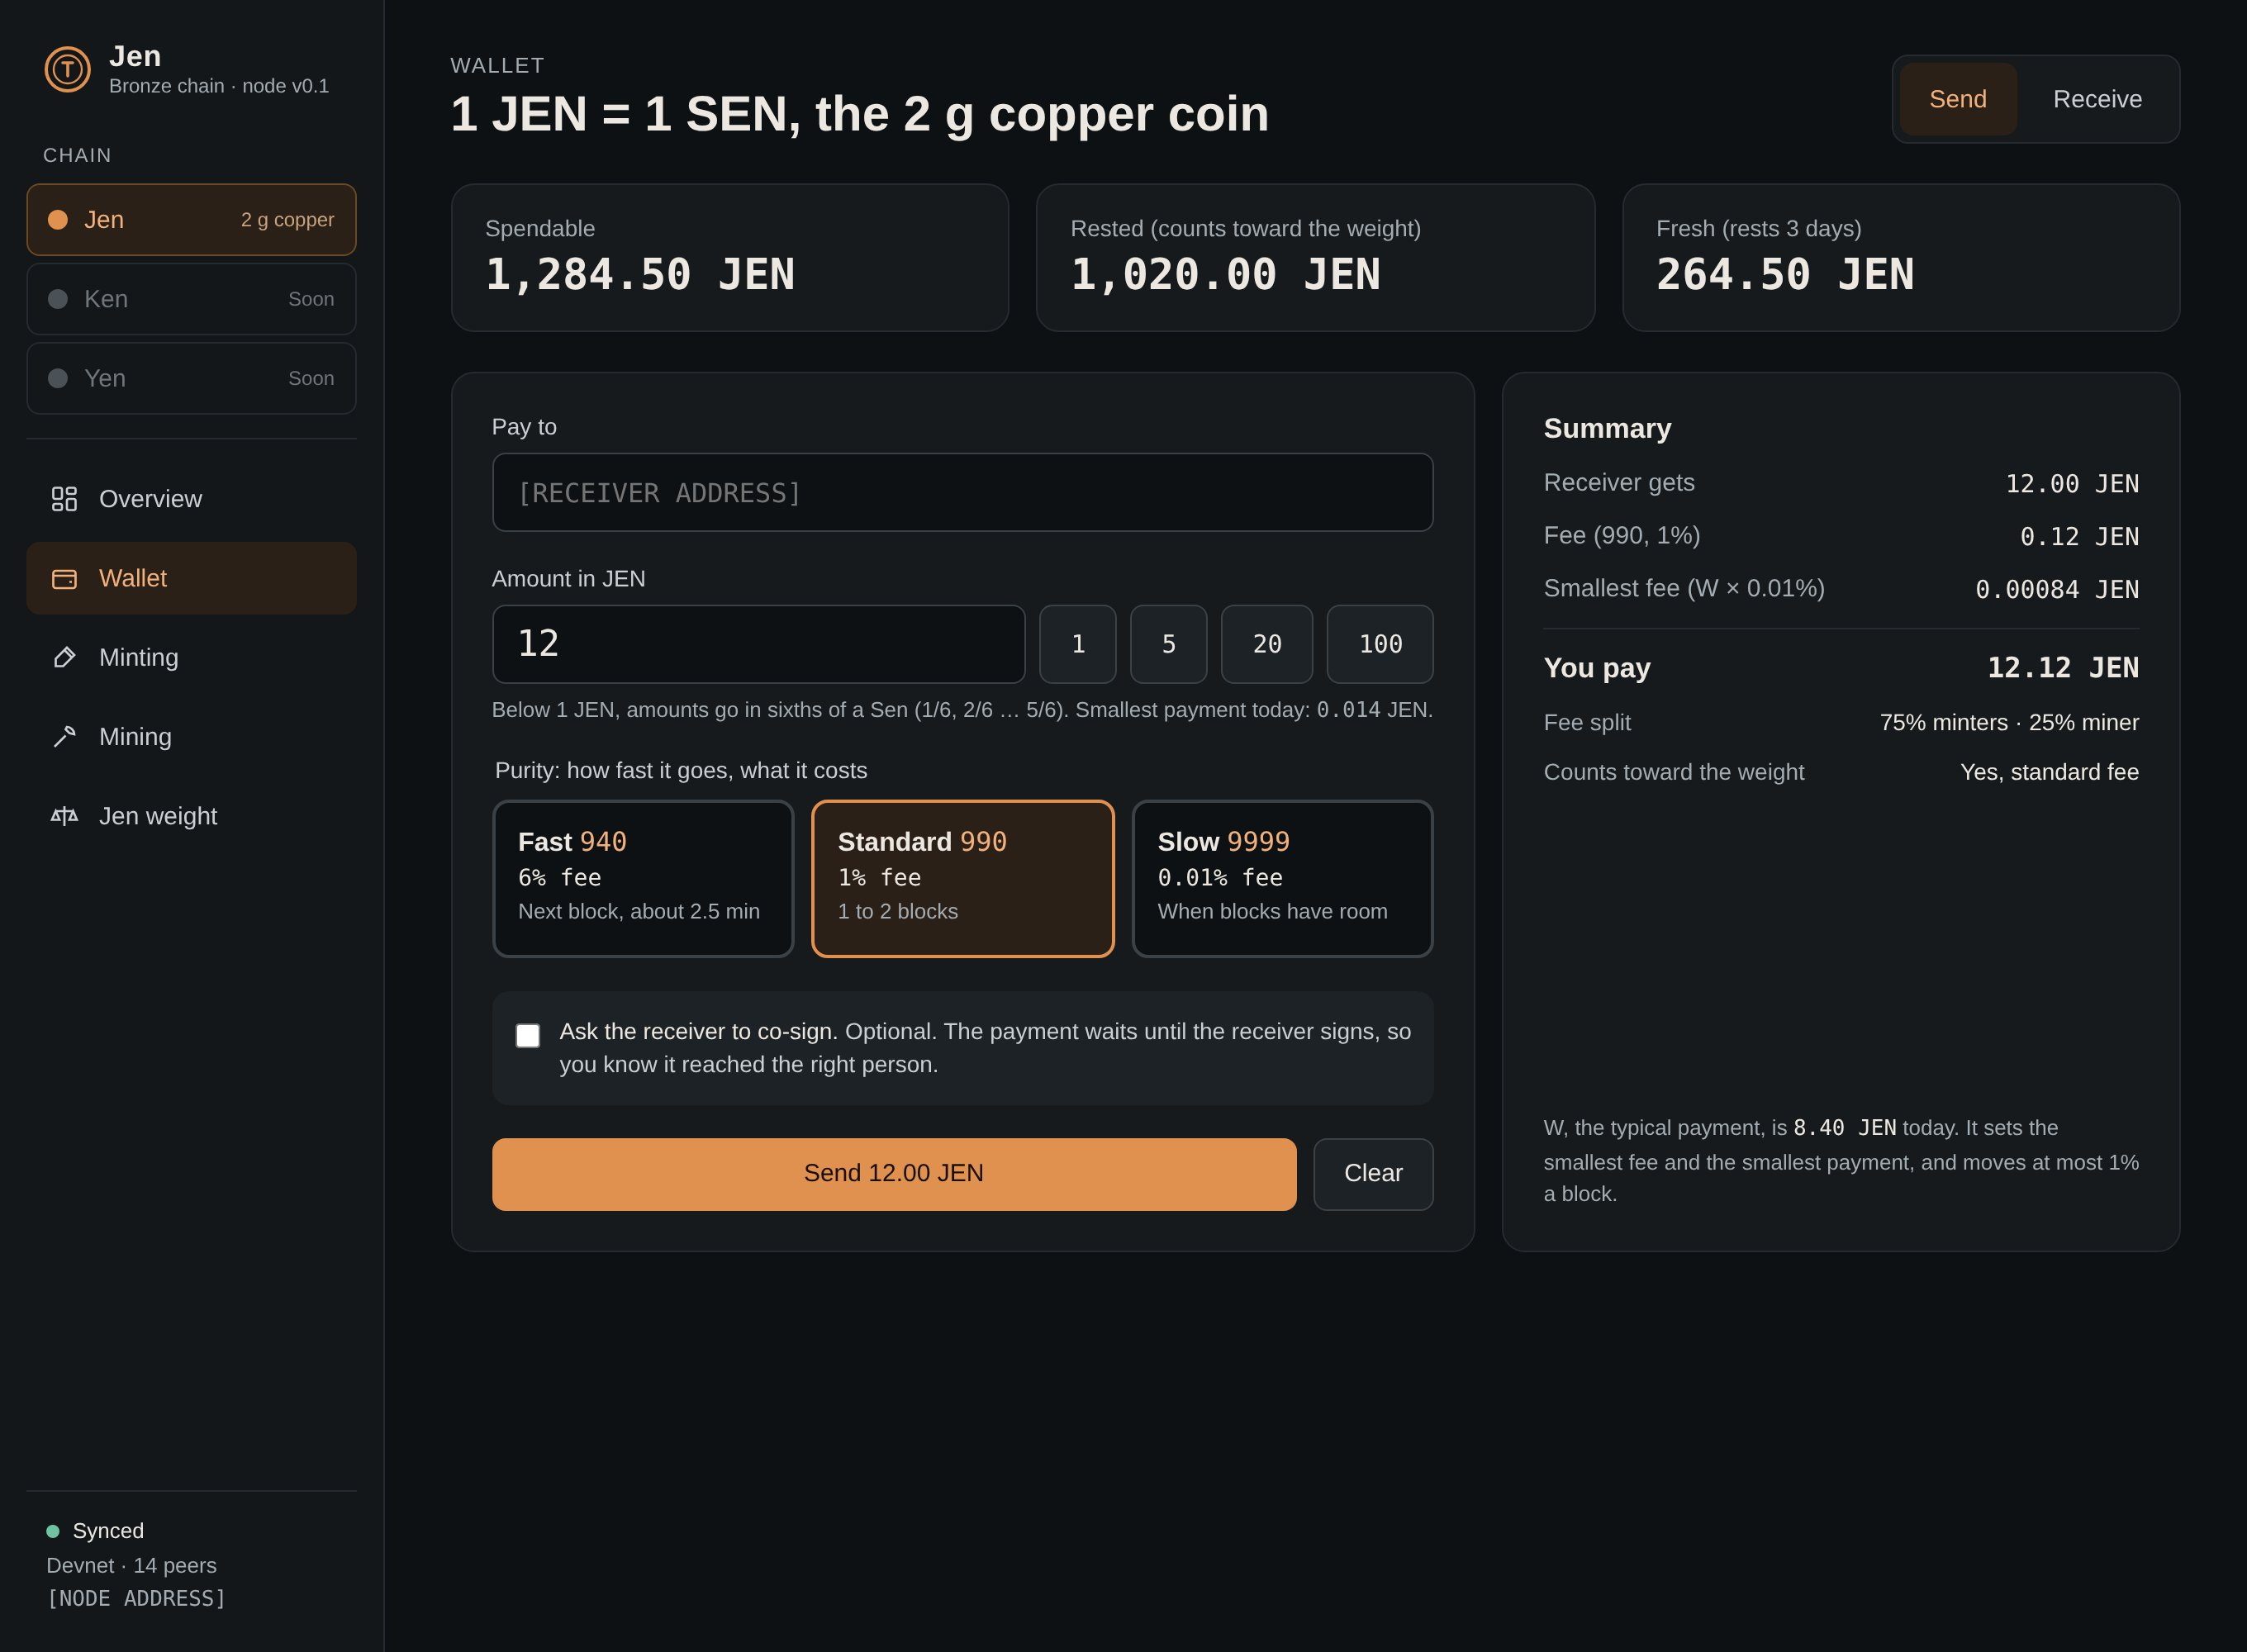
\includegraphics[width=0.98\textwidth]{figs/ui_wallet.jpg}
\caption{Wallet: amount in \JEN{} (sixths below 1), purity choice, optional receiver co-signature, and the fee worked out from the purity and the amount.}
\end{subfigure}\\[8pt]
\begin{subfigure}{0.70\textwidth}\centering
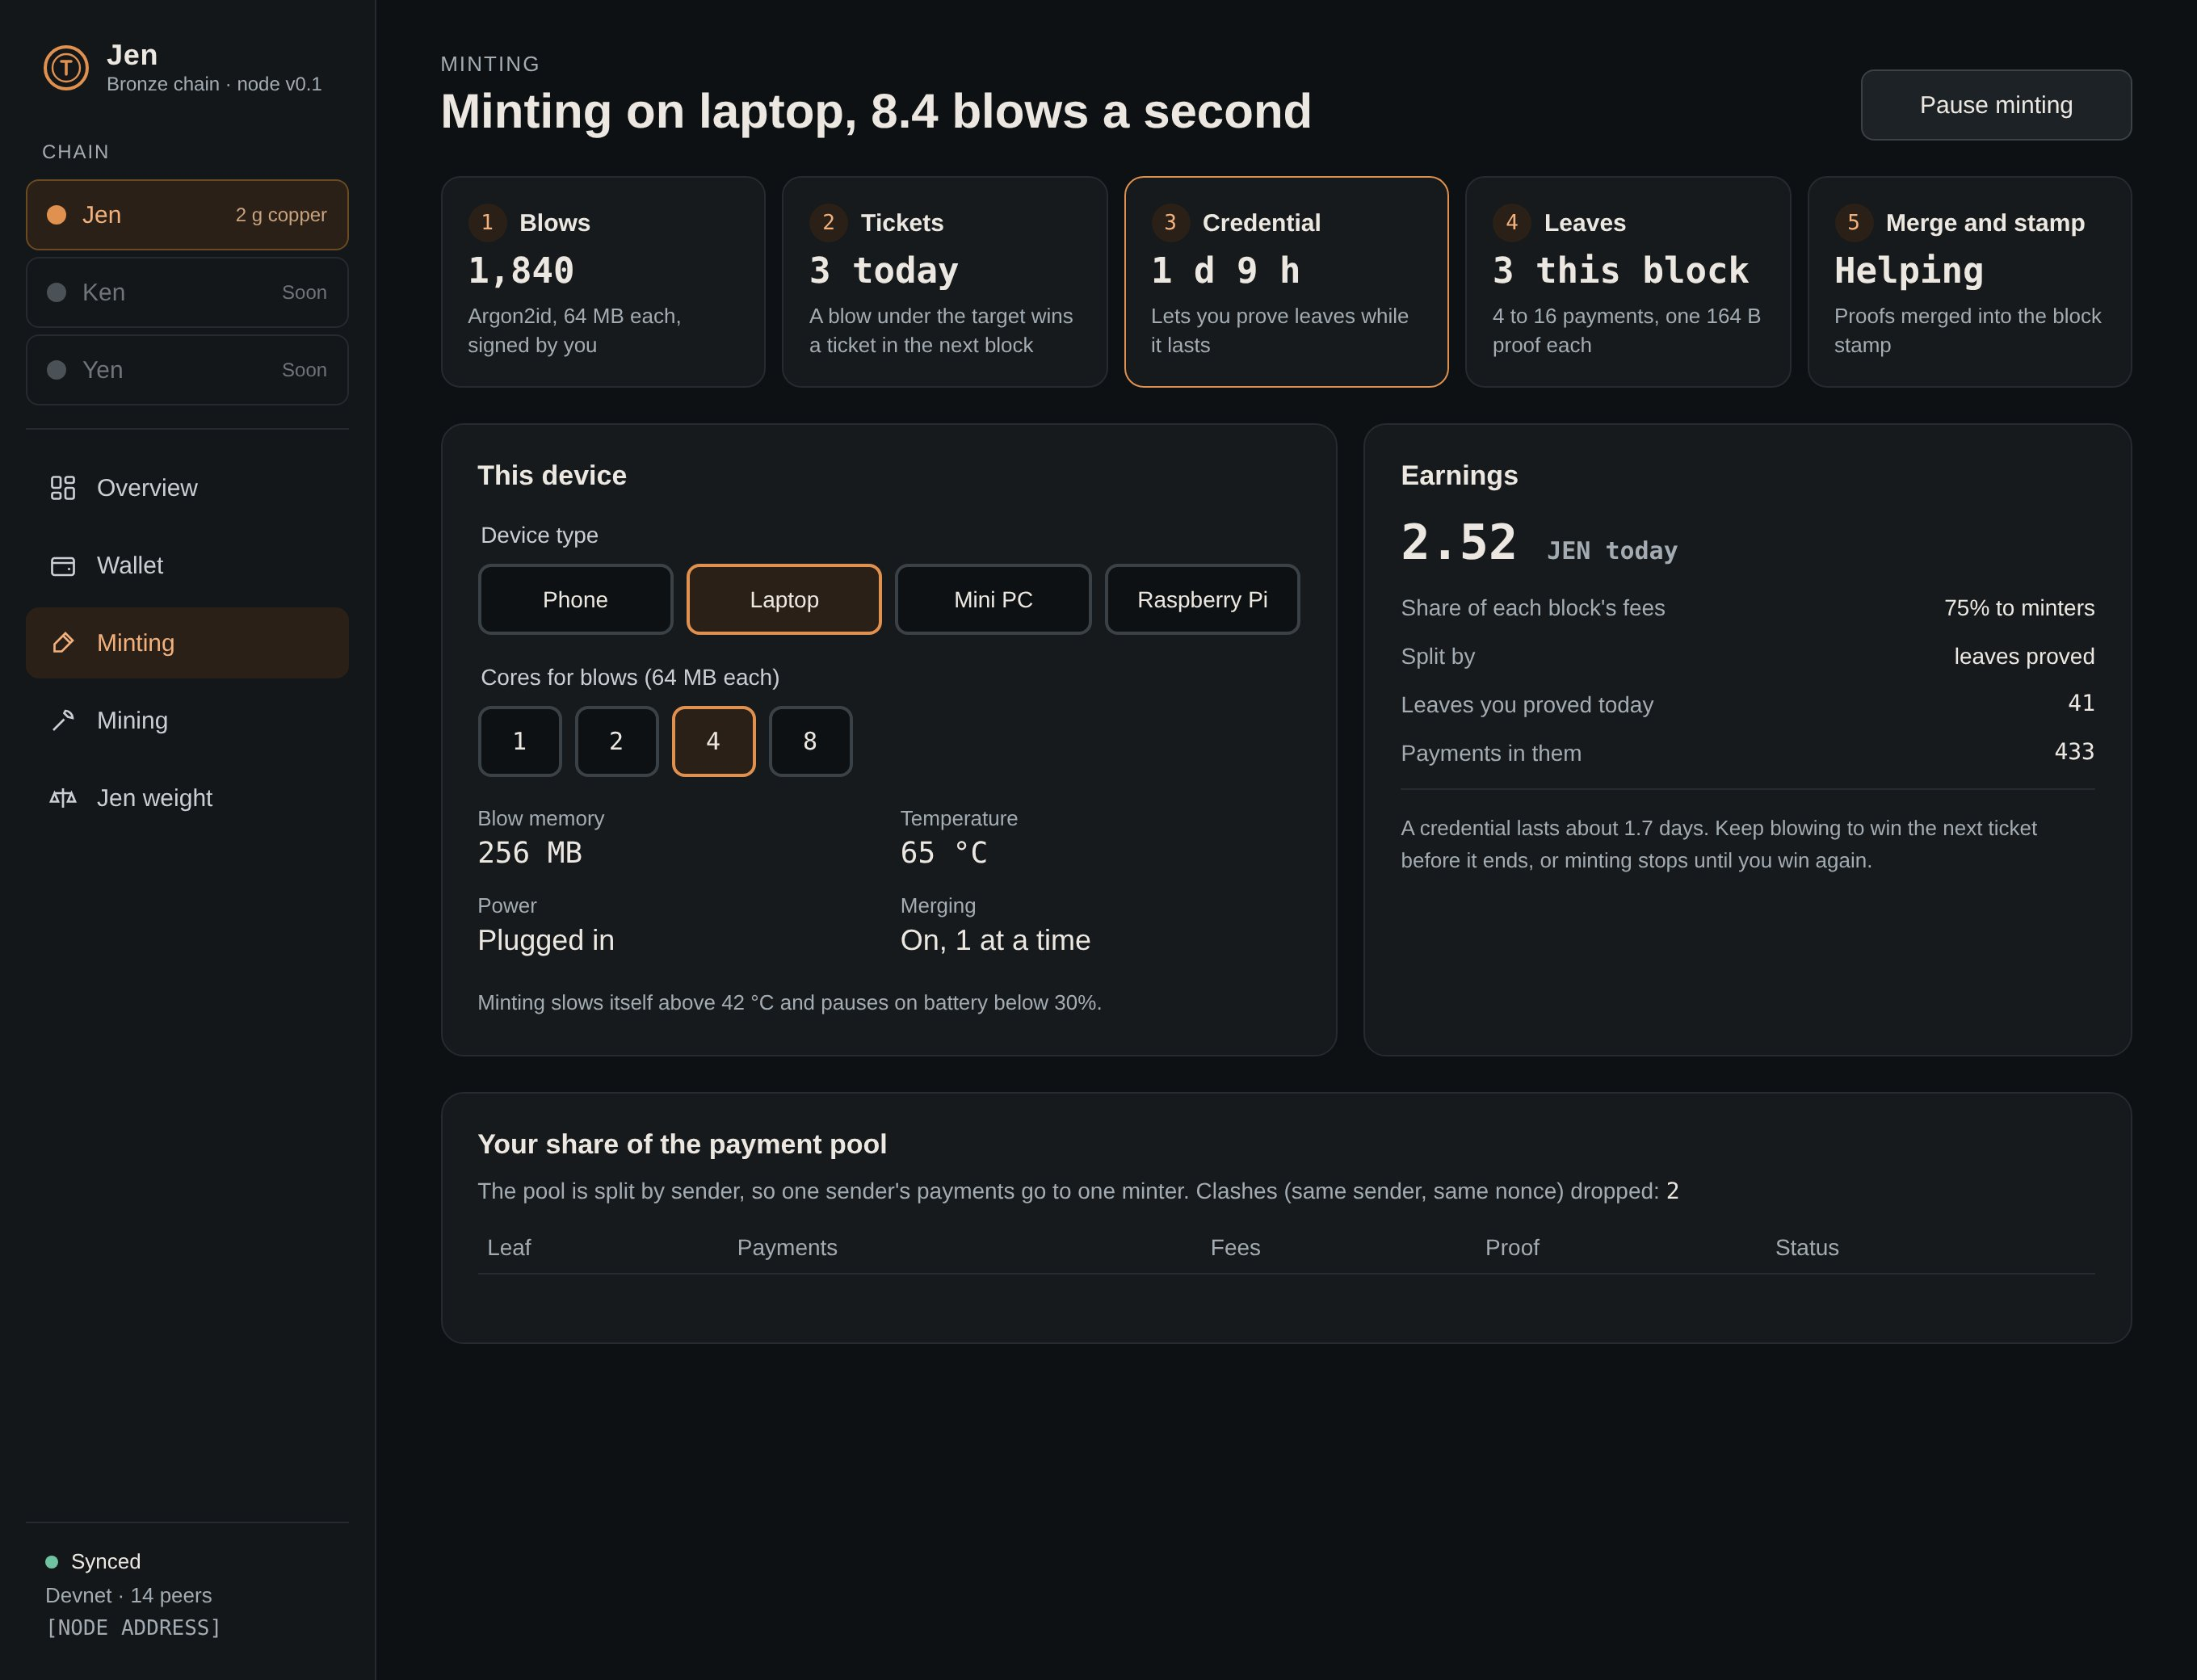
\includegraphics[width=\textwidth]{figs/ui_mint.jpg}
\caption{Minting: blows, tickets, credential, leaves and merging; device type and cores; the payment pool split by sender.}
\end{subfigure}\hfill
\begin{subfigure}{0.26\textwidth}\centering
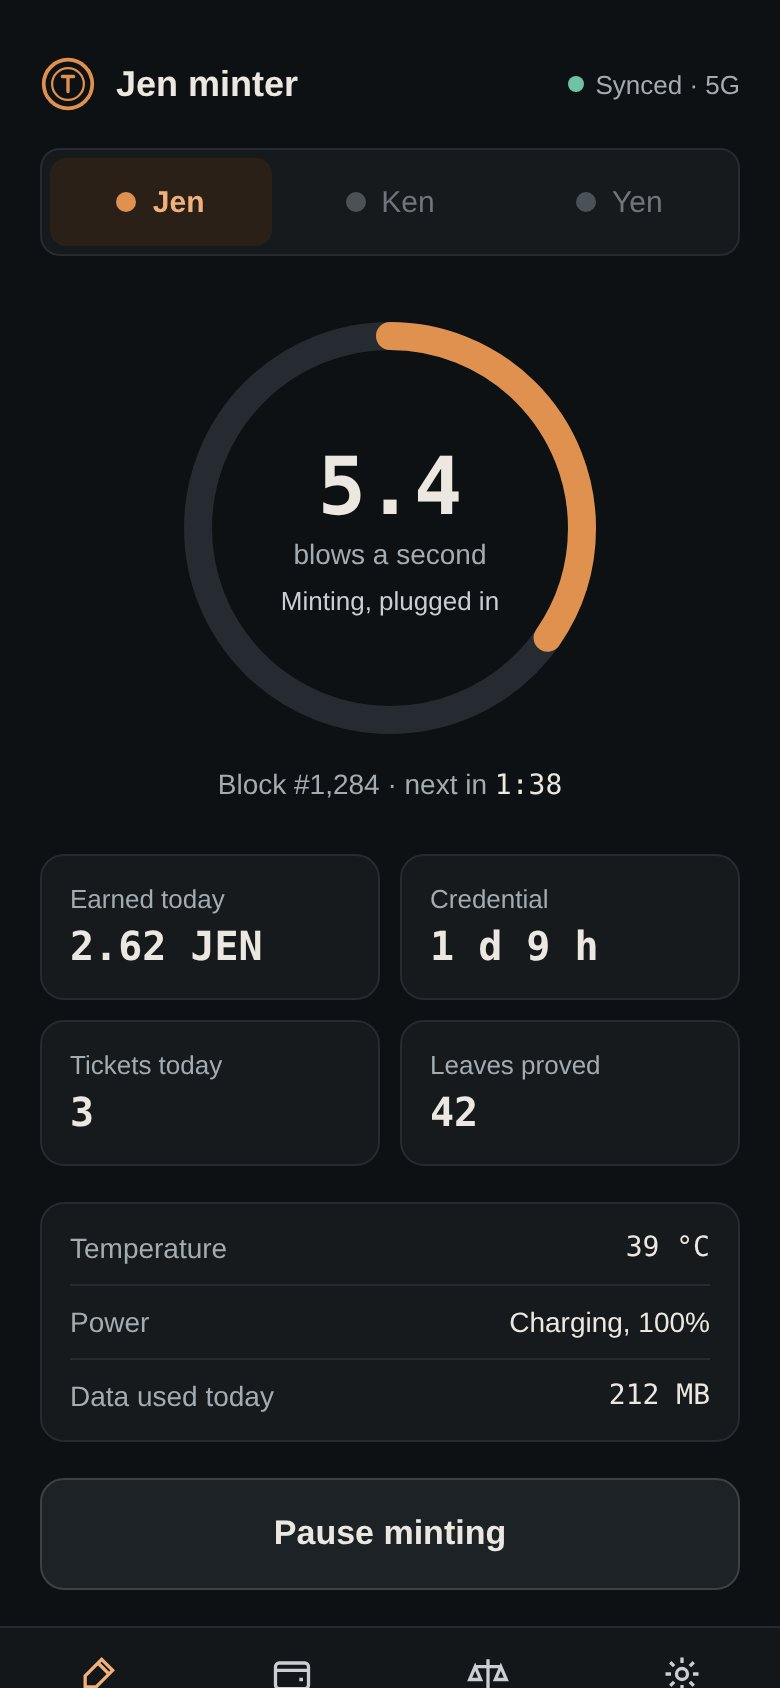
\includegraphics[width=\textwidth]{figs/ui_phone.jpg}
\caption{Phone minter (Android).}
\end{subfigure}
\caption{The Jen v1 interface prototype (sample data). Continued in Figure~\ref{fig:ui2}.}
\label{fig:ui}
\end{figure}

\begin{figure}[tbp]
\centering
\begin{subfigure}{\textwidth}\centering
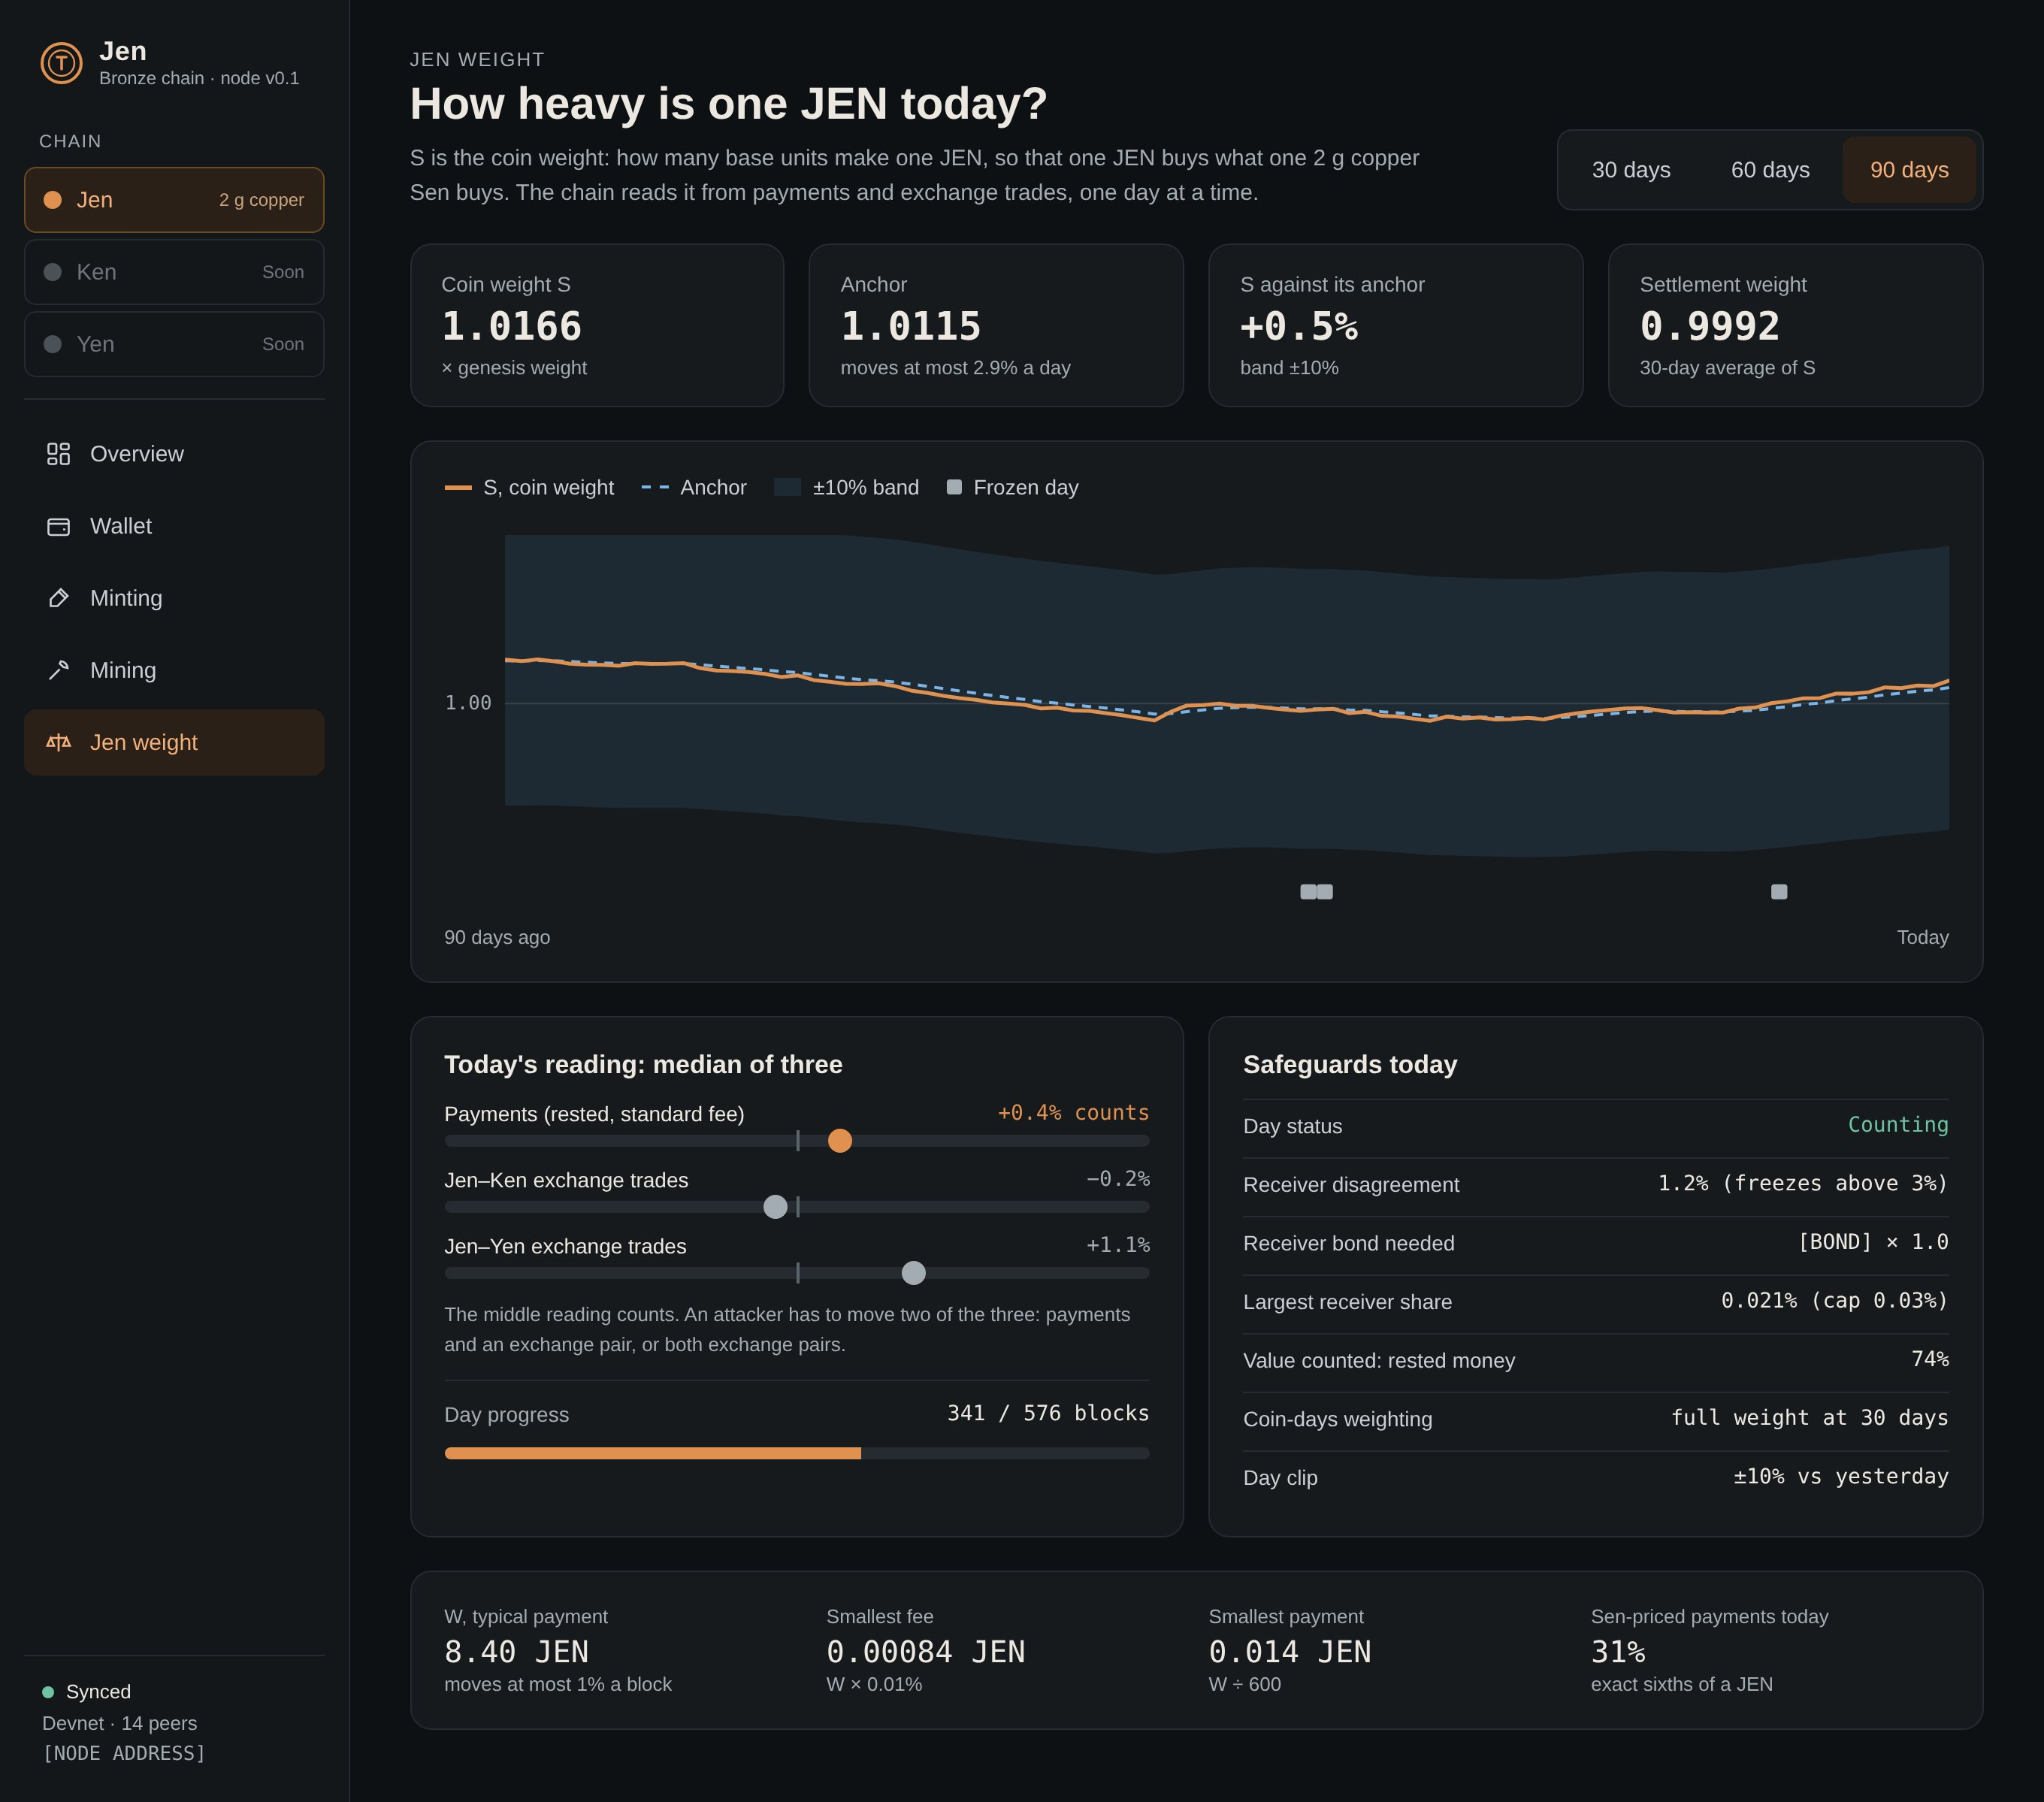
\includegraphics[width=0.98\textwidth]{figs/ui_weight.jpg}
\caption{Jen weight: $S$ against its anchor and band, today's three readings, the safeguards and the fee measure ($W$, since removed, Section~\ref{sec:w}).}
\end{subfigure}\\[8pt]
\begin{subfigure}{0.49\textwidth}\centering
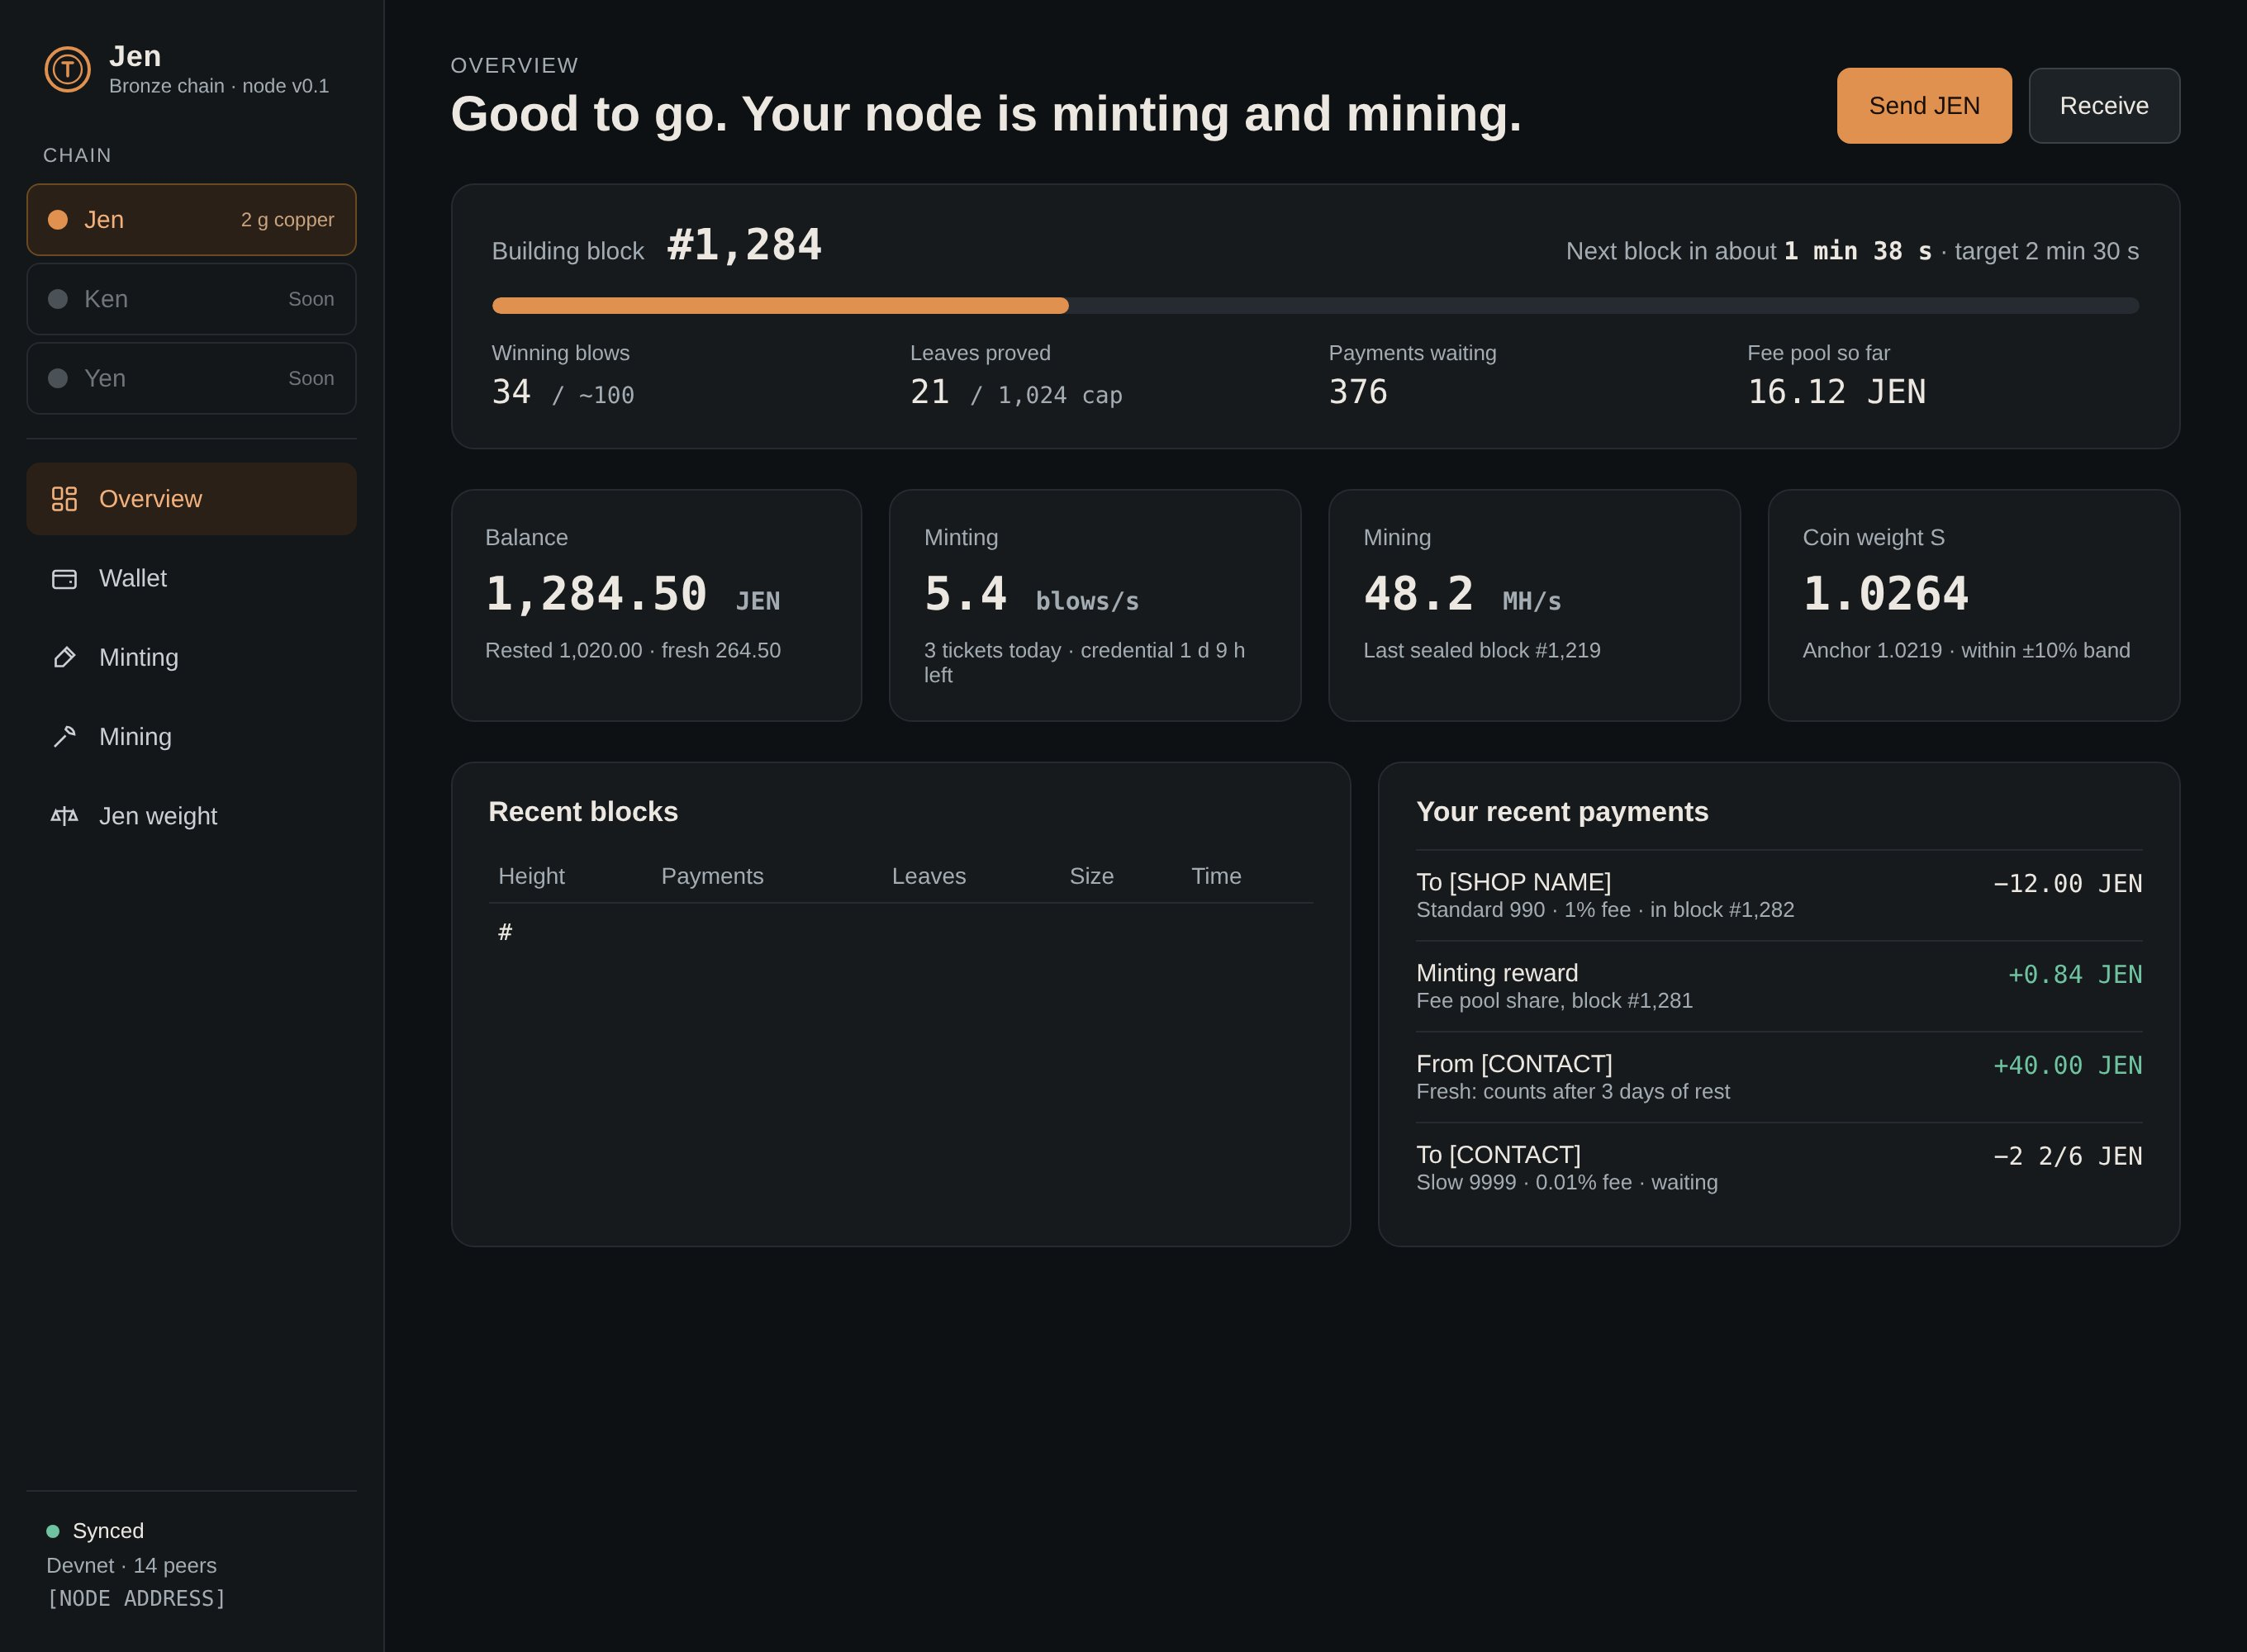
\includegraphics[width=\textwidth]{figs/ui_main.jpg}
\caption{Overview.}
\end{subfigure}\hfill
\begin{subfigure}{0.49\textwidth}\centering
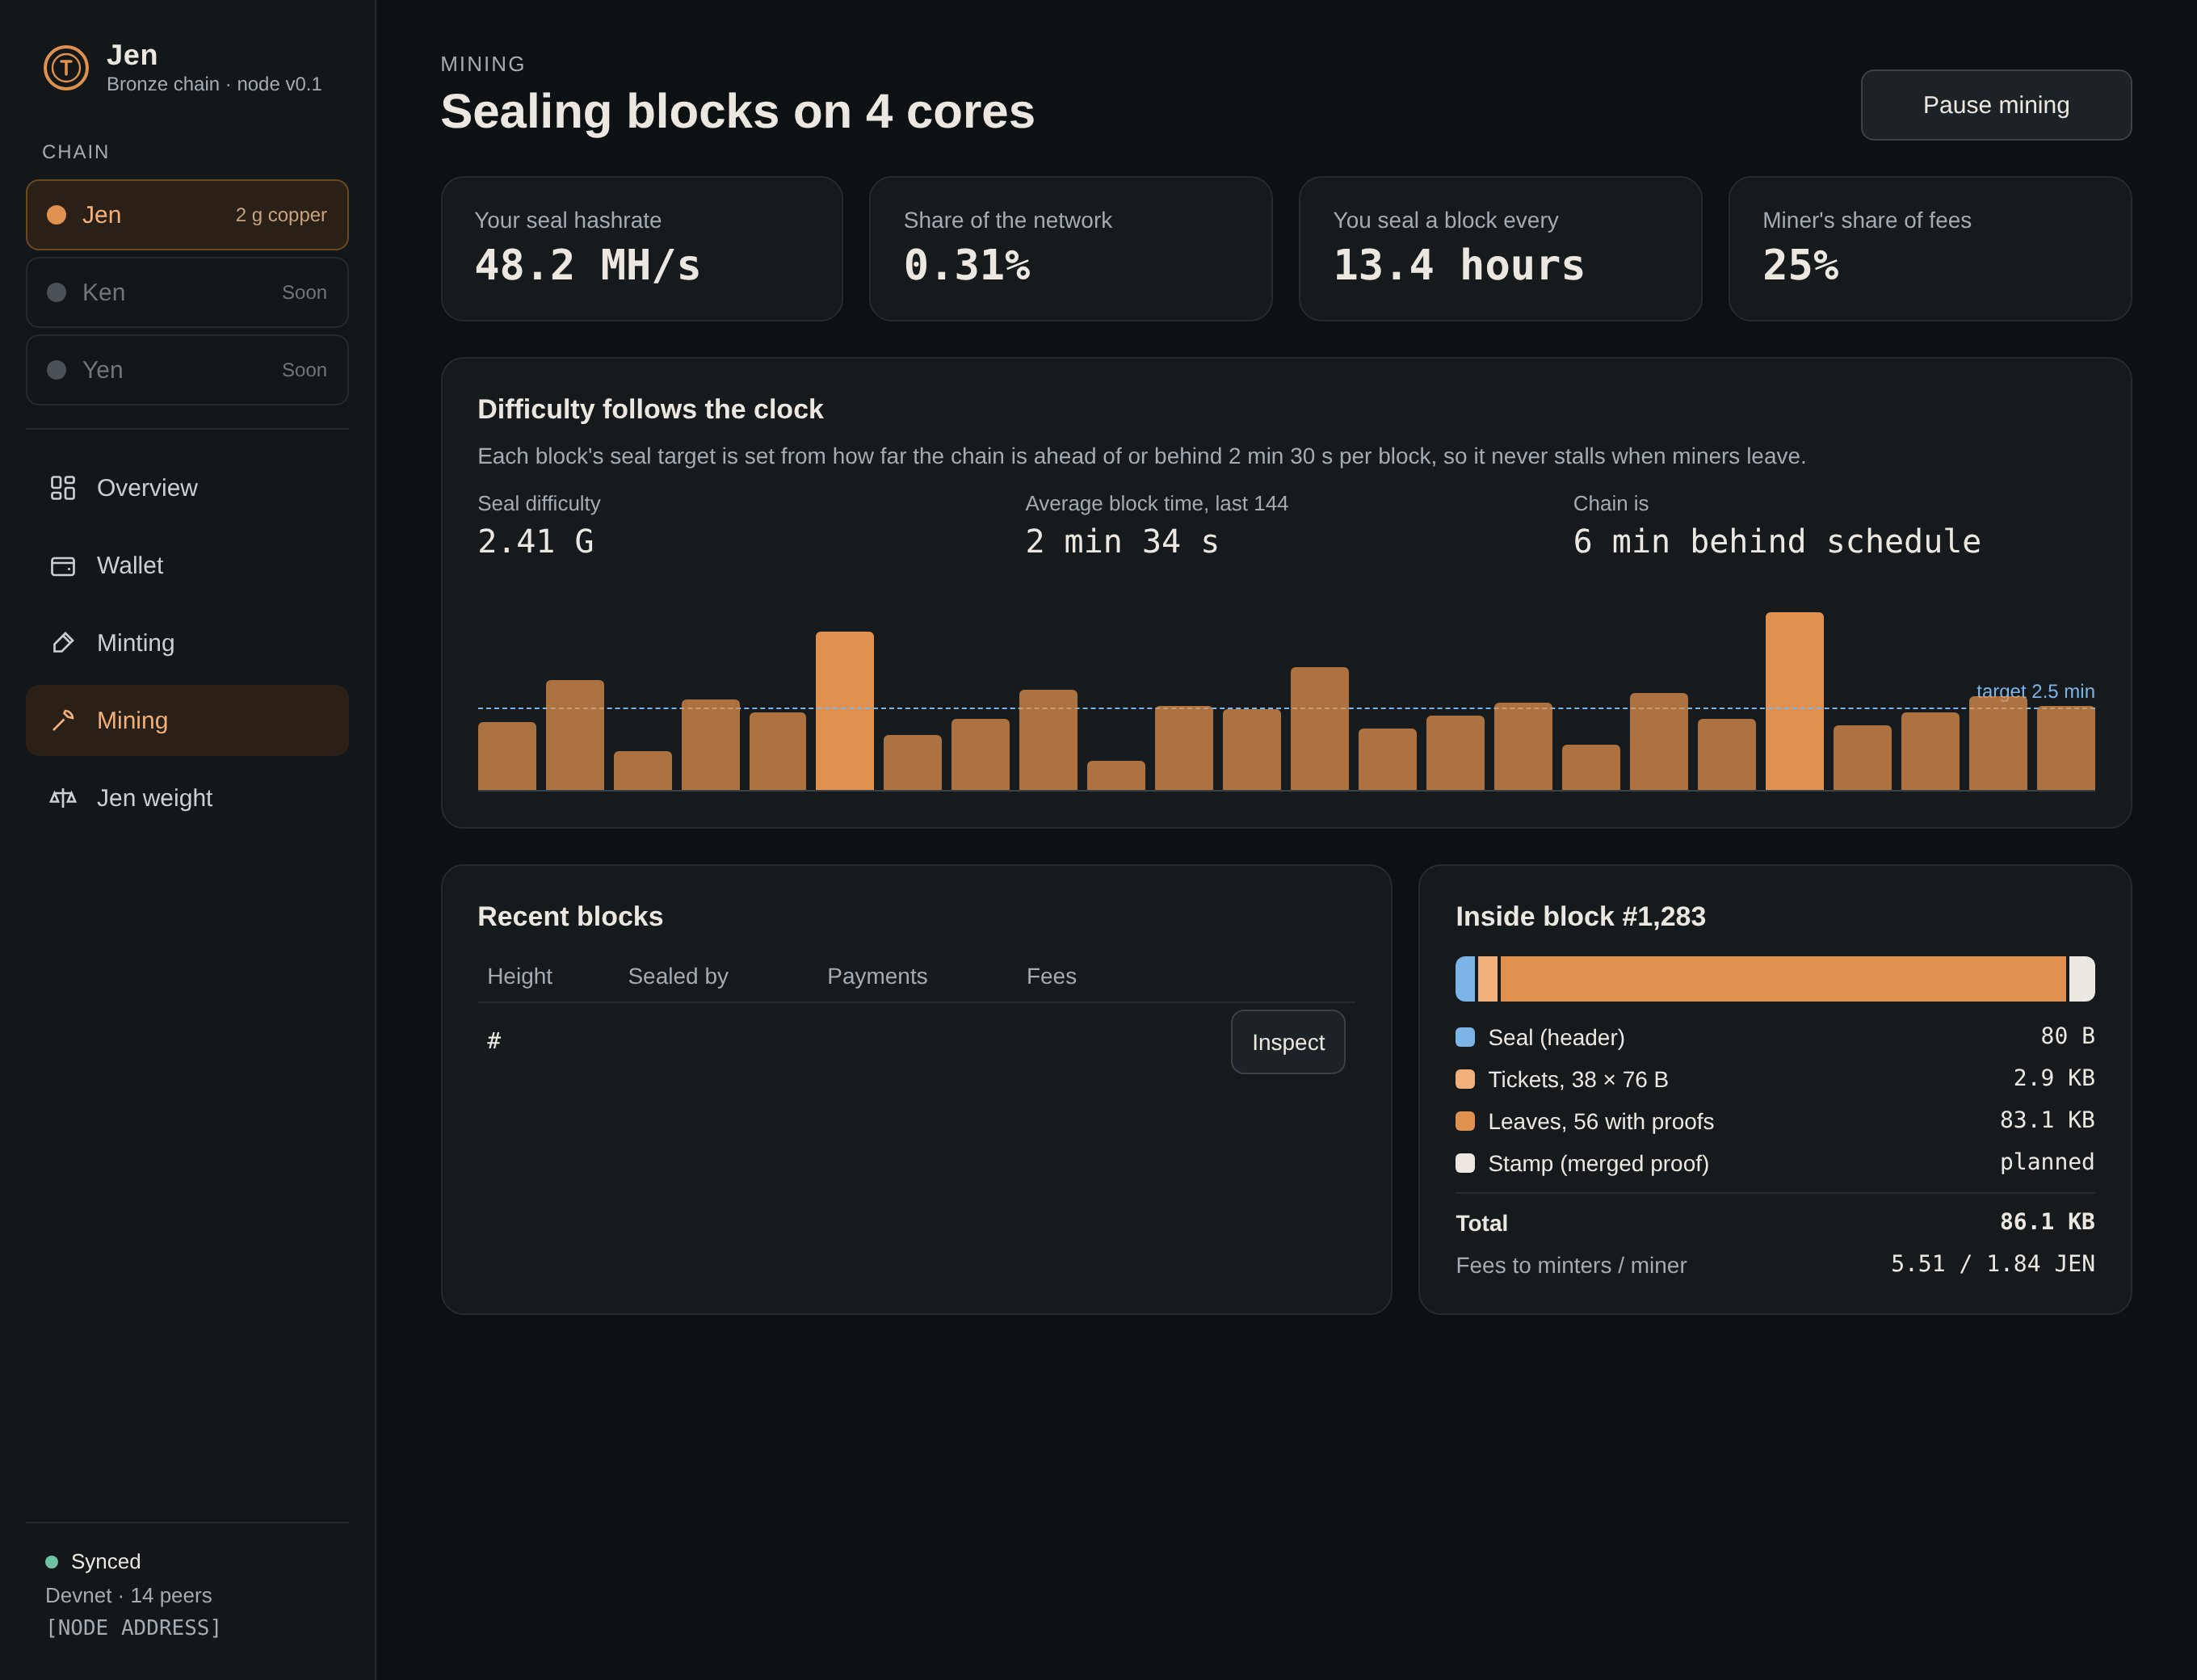
\includegraphics[width=\textwidth]{figs/ui_mine.jpg}
\caption{Mining: seal hashrate, time-based difficulty, block contents.}
\end{subfigure}
\caption{The Jen v1 interface prototype, continued.}
\label{fig:ui2}
\end{figure}

%=====================================================================
\FloatBarrier
\section{Economics and related work}\label{sec:econ}

\paragraph{Three roles separated.} Zen separates three roles that metal money historically combined. Physical coins of fixed weight are a store of value held privately. Electronic coins are the medium of payment. Each chain's $S$ states the electronic coin's value in grams of its metal.

\paragraph{Small change.} For centuries full-weight small coins were chronically scarce because they cost relatively more to mint \cite{sargentvelde}. The electronic Jen supplies small change in sixths of a Sen, at no minting cost, and in fractions of that over channels.

\paragraph{Fisher's compensated dollar.} Irving Fisher proposed fixing nothing but the dollar's purchasing power and varying its gold weight each month, with a 1\% spread so speculation could not profit \cite{fisher1914,fisher1920}; a modern comparison finds it would have cut price uncertainty by an order of magnitude \cite{bordo}. Zen follows the same logic in reverse: the stamped coins stay fixed, the electronic unit's weight floats with what the metal buys, and the anchor and band play the role of Fisher's spread.

\paragraph{Lessons from failed self-regulating money.} Designs that defended a peg by minting a second token failed through self-reinforcing runs: Terra (about \$50bn, May 2022) \cite{terra}, Iron Finance \cite{ironfinance}, Basis Cash \cite{basiscash} and NuBits \cite{nubits}. Zen has no second token defending a price and no collateral to liquidate, so its failure mode is mismeasurement or drift, not a death spiral. Three lessons still apply: lagging prices must not trigger automatic conversions (hence settlement at the 30-day average); coin age is useful but can be saved up and spent at once (held here by the cap, the middle-20\% reading and the band); and thin markets are cheap to move \cite{mango,uniswap}, hence a minimum exchange volume and a discount for payments created by the block's own producers (open).

\begin{table}[htbp]
\centering\footnotesize
\begin{tabularx}{\textwidth}{>{\raggedright\arraybackslash}p{3.0cm} Y Y Y}
\toprule
\textbf{Family} & \textbf{Examples} & \textbf{Where trust sits} & \textbf{Difference from Zen}\\
\midrule
Metal held by a custodian & e-gold, PAX Gold, Tether Gold & custodian, auditor & Zen's coin is not a claim on anyone's metal\\
Collateral + price feed & BitShares, Synthetix sXAU & feed publishers & no collateral, no feed\\
Rebasing to a target & Ampleforth & external oracle & input is the chain's own payments\\
Price from own payments & UTXOracle, brk\_oracle & nobody; outside consensus & read inside consensus, with a protocol grid (sixths) and defences\\
Staked reporters & SchellingCoin, UMA, Chainlink & stake-weighted reporters & no reporters to bribe\\
Issuance from history & Komi \& Tatekawa & consensus & steers issuance, sets no peg\\
Commodity money in theory & Fisher, Hayek, Graham, Keynes & a mint or buffer stock & no agent; the weight floats by consensus\\
\bottomrule
\end{tabularx}
\caption{Related work \cite{egold,paxg,bitusd,synthetix,ampleforth,utxoracle,brk,schellingcoin,komi,hayek,ussher}. The novelty claim rests on a limited literature search with no patent search and means ``no prior design found''.}
\label{tab:related}
\end{table}

%=====================================================================
\section{Security summary}\label{sec:security}

\begin{center}\begin{minipage}{\textwidth}\centering
\centering\small
\begin{tabularx}{\textwidth}{l Y Y}
\toprule
\textbf{Attack} & \textbf{Defence} & \textbf{Evidence}\\
\midrule
Stealing or outsourcing blows & each blow is signed by the minter's key & forged proofs and stolen blows rejected (simulation, 1,000 minters; devnet)\\
Forged leaf proof & proofs verified by every node; public inputs bind state roots, fees, prover & rejected on devnets with real proofs\\
Double spend via two minters & rank order; the state leaf skips a used (sender, nonce) & devnet supply exact; skipped in the Rust block (measured)\\
Builder changing a signed payment & state leaf re-hashes the signed fields against the signature leaf & no proof produced (measured)\\
Builder paying itself or others too much & nodes recompute the payout list; credits must match exactly & block rejected (measured)\\
Reusing a seal or swapping the miner address & commitment covers the coinbase and the body & rejected (measured)\\
A lock operation the node refuses & each operation family has its own circuit; the merge accepts only their four keys & 583 rule-breaking tries, none proves a refused operation (testnet)\\
A claim without a real foreign payment & every node checks the payment proof; the stamp binds its digest to the claim and the signature & rejected if the proof is wrong; not checked inside the stamp (testnet)\\
Overflowing a balance check & balance, amount and fee compared in 128-bit integers; money values below $2^{62}$ in circuits & wrapped sum refused (testnet, internal review)\\
Replaying a vault claim on another chain & the chain id is in the signed message & refused on the other chain (testnet)\\
Copying a sealed network request & one-time key kept in a replay cache for two time windows & copy inside the window refused (testnet)\\
A heavier-looking chain with less work & cross-chain follower keeps the chain with most cumulative work & rule tested (testnet)\\
Forged signature & checked inside the leaf proof, $s<n$, no exceptional curve cases & no proof produced (measured)\\
Replaying a signed payment & nonce in the signed message, incremented by the proof & no proof produced (measured)\\
Withholding or changing block data & stamp commits to a hash of the payments; nodes replay them & one changed byte rejected (measured)\\
Reusing a stamp for another block & public values bind roots, fees, count and data & rejected by the Groth16 verifier (measured)\\
One prover filling blocks & leaf quota and split pool & 15$\times$ faster prover: 99\% $\to$ 23\% of leaves (devnet)\\
Hidden chain with sealing power & two-factor fork choice & 3$\times$ sealing, 50\% minting: 59\% of honest weight (devnet)\\
Lowering one's own blow difficulty & gate and fork choice by minting work & attacker reached 58\% of honest work (devnet)\\
Faking congestion to resize & fee pool paid forward; grow only when full & --\\
Pushing $S$ & layered defences (Table~\ref{tab:layers}) & $\le$13\%/week; \$0.5M/month at 12\% (simulated)\\
Locking out small payers & fee limits in coins (0.01 coin; $\tfrac16$~\JEN{} smallest payment), not in typical payment sizes & --\\
Launch stall & time-based difficulty & block 100 in 10 h instead of 28 h (simulated)\\
\bottomrule
\end{tabularx}
\captionof{table}{Attacks and defences across the system.}
\end{minipage}\end{center}

%=====================================================================
\FloatBarrier
\section{Open problems and roadmap}\label{sec:open}

\begin{enumerate}
\item \textbf{The stamp in production.} Benchmarked (Section~\ref{sec:stamp}): one 196-byte proof per block, with signatures inside. Done: one key for every block size (a universal merge circuit), new and closed accounts, the chain id and prover credits inside the circuit, split signature and state leaves, one key per person for payments and blows, payouts inside the proof, the peg's account fields in the leaf, a Bitcoin-exact seal for Stratum pools, the rule that every block carries its stamp, and, on the Rust test network, every lock operation (vault, channel, order with auctions and claim, factory) inside the same stamp, with a soundness battery of 583 tries. Still open: a \textbf{public multi-party Groth16 ceremony} for the final circuit (the test key was made by one machine and is not safe for value), the foreign payment proof of an order claim inside the circuit, a builder benchmark on a many-core GPU server, phone proving tests, fuzzing of every decoder, and an external audit of circuits and consensus. The 70\,KB Plonky2 stamp, which needs no ceremony, is the fallback.
\item \textbf{The young chain.} Jen runs alone for about 3.5 years with little traffic and no exchange: a slower anchor, a longer rest and a lower cap while volume is low, a launch simulation, and the time-based difficulty for blows and seals.
\item \textbf{Faster honest following.} When payments and both exchange readings agree on a move, let the anchor move faster (for example 3 times); an attacker cannot fake all three at once.
\item \textbf{Ordinary-side attacks.} Fake ordinary payments (the gram side of the reading) are not yet simulated.
\item \textbf{Block producers.} Discount payments created by the block's own miner or minter, and count rest periods in blocks.
\item \textbf{Channels and the sample.} Payments kept in channels never reach the reading, so the sample shrinks and skews toward large flows as channels succeed. Which channel events count as observations is open.
\item \textbf{Thin exchange pairs.} A minimum daily volume before an exchange reading counts.
\item \textbf{Adaptive attackers.} Aged balances spent at once, switching direction when defenders arrive, staying just under each trigger.
\item \textbf{Pricing practice.} Wallets that quote coin prices and ratios from metal prices by default, since the peg converges only when most coin-priced value is set from the metal.
\item \textbf{A formal bound.} A cost-of-corruption bound for the peg, as Bitcoin states the attacker's catch-up probability.
\item \textbf{Open parameters.} Whether $V$ applies to Yen's first blocks; the reward curve (smooth or step table); the fee split as rewards fade; leaf size at launch; the seal hash; and the exchange version at launch (Table~\ref{tab:opendec}).
\end{enumerate}

\begin{table}[htbp]
\centering\small
\begin{tabularx}{\textwidth}{Y Y Y}
\toprule
\textbf{Question} & \textbf{Options} & \textbf{Recommendation}\\
\midrule
Random factor in Yen's first blocks & random from block 1, or $V=1$ for $\approx$100 blocks & fixed at first\\
Reward curve & smooth (Yen limit $\approx$7,255) or step table (10,080) & smooth curve\\
Fee split minters / miner & fixed 75/25, or miner share rising as the reward fades & rising miner share\\
Leaf size at launch & 4, 8 or 16 payments & 4 for phones, 16 for desktops\\
Proof system & Plonky2 leaves and merges wrapped in one Groth16 stamp (ceremony), or the 70\,KB Plonky2 stamp (no setup) & Plonky2 + Groth16 stamp, with a public ceremony\\
Hash inside proofs & MiMC, Poseidon or Poseidon2 & Poseidon over Goldilocks; over BN254 in the last layer\\
Seal hash & SHA-256 or a hash that resists dedicated chips & to research\\
Exchange at launch & reserve--pay--claim, or batch auctions & reserve--pay--claim first\\
\bottomrule
\end{tabularx}
\caption{Open decisions (specification 11).}
\label{tab:opendec}
\end{table}

%=====================================================================
\section{Conclusion}
Zen proposes metal money with no vault and no price feed. Three physical coins set the reference; three chains read their value from the way people pay, and defend that reading with rules whose cost to an attacker can be measured. Phones mint the blocks and share the fees, ordinary SHA-256 hardware seals them, and channels, the exchange and Zen Net carry the payments that do not need to be on a chain. The simulations in this paper suggest that the peg can be made expensive to move and quick to restore, provided most coin-priced shops price from the metal itself. A Rust implementation now runs the three chains on a test network, with the merge proof carrying payments and every lock operation. The next steps are a public Groth16 ceremony, fuzzing and an outside audit, a launch simulation, and a public testnet open to phones.

\paragraph{Author's note.} Zen, its six coins (Gold Ren, Silver Ten and Copper Sen; Golden Yen, Silver Ken and Bronze Jen) and the designs in this paper are the work of Justus L. Ludovic. Prototype code: the Rust node \texttt{zenproof} (rounds 1 to 55), \texttt{zen\_minting.py}, \texttt{pom\_simulation.py}, \texttt{pom-leaf} (Go, gnark), the Jen-0 to Jen-0.11 devnets and the peg simulations listed in Appendix~\ref{app:sims}.

%=====================================================================
\begin{thebibliography}{99}\small
\setlength{\itemsep}{1pt}
\bibitem{nakamoto} S.~Nakamoto, \emph{Bitcoin: A Peer-to-Peer Electronic Cash System}, 2008. \url{https://bitcoin.org/bitcoin.pdf}
\bibitem{yermack} D.~Yermack, \emph{Is Bitcoin a Real Currency? An Economic Appraisal}, NBER w19747, 2013. \url{https://www.nber.org/papers/w19747}
\bibitem{klagesmundt} A.~Klages-Mundt, D.~Harz, L.~Gudgeon, J.-Y.~Liu, A.~Minca, \emph{Stablecoins 2.0}, AFT 2020. \url{https://arxiv.org/pdf/2006.12388v2}
\bibitem{caldarelli} G.~Caldarelli, \emph{Understanding the Blockchain Oracle Problem}, Information 11(11), 2020. \url{https://www.mdpi.com/2078-2489/11/11/509/htm}
\bibitem{douceur} J.~R.~Douceur, \emph{The Sybil Attack}, IPTPS 2002. \url{https://www.microsoft.com/en-us/research/publication/the-sybil-attack/}
\bibitem{egold-doj} US Department of Justice, e-gold plea, July 2008. \url{https://www.justice.gov/archive/opa/pr/2008/July/08-crm-635.html}
\bibitem{egold} e-gold (overview). \url{https://en.wikipedia.org/wiki/E-gold}
\bibitem{paxg} Gold-backed stablecoins overview (PAXG, XAUt, KAU). \url{https://stablecoininsider.org/gold-backed-stablecoins/}
\bibitem{bitusd} The Block, \emph{bitUSD loses its peg}, 2019. \url{https://www.theblock.co/news/markets/2019-02-15-bitusd-hasnt-had-its-1-peg-for-more-than-two-months-11876}
\bibitem{synthetix} Synthetix, Chainlink price feeds for sXAU/sXAG. \url{https://blog.synthetix.io/chainlink-decentralizes-first-wave-of-synthetix-price-feeds/}
\bibitem{ampleforth} Chainlink, Ampleforth case study. \url{https://chain.link/case-studies/ampleforth}
\bibitem{utxoracle} UTXOracle: a decentralized approach to the oracle problem. \url{https://www.nasdaq.com/articles/utxoracle:-a-decentralized-approach-to-the-oracle-problem}
\bibitem{brk} brk\_oracle documentation. \url{https://docs.rs/crate/brk_oracle/0.3.4}
\bibitem{schellingcoin} V.~Buterin, \emph{SchellingCoin}, 2014. \url{https://blog.ethereum.org/2014/03/28/schellingcoin-a-minimal-trust-universal-data-feed}
\bibitem{komi} Komi \& Tatekawa, \emph{Consensus Algorithm Using Transaction History}, ePrint 2023/373. \url{https://eprint.iacr.org/2023/373.pdf}
\bibitem{nubits} Moneyness, \emph{The end of a stablecoin} (NuBits), 2016. \url{https://www.moneyness.ca/2016/08/end-of-stablecoin.html}
\bibitem{mango} Davis Wright Tremaine, CFTC action on Mango Markets, 2023. \url{https://dwt.com/blogs/financial-services-law-advisor/2023/01/cftc-decentralized-manipulation-crypto}
\bibitem{terra} J.~Liu, I.~Makarov, A.~Schoar, \emph{Anatomy of a Run: The Terra Luna Crash}, NBER w31160. \url{https://www.nber.org/papers/w31160}
\bibitem{ironfinance} Finematics, \emph{Bank run in DeFi: Iron Finance explained}. \url{https://finematics.com/bank-run-in-defi-iron-finance-explained/}
\bibitem{basiscash} Zhao, Li \& Yuan, Basis Cash model checking, arXiv 2101.08423. \url{https://ar5iv.arxiv.org/html/2101.08423}
\bibitem{peercoin} S.~King, S.~Nadal, \emph{PPCoin: Peer-to-Peer Crypto-Currency with Proof-of-Stake}, 2012. \url{https://raw.githubusercontent.com/papers-we-love/papers-we-love/refs/heads/main/digital_currency/peercoin.pdf}
\bibitem{uniswap} Uniswap Labs, \emph{Uniswap v3 TWAP oracles in proof of stake}. \url{https://blog.uniswap.org/uniswap-v3-oracles}
\bibitem{velde} F.~Velde, \emph{The Crime of 1873: Back to the Scene}, Chicago Fed WP 2002-29. \url{https://www.chicagofed.org/~/media/publications/working-papers/2002/wp2002-29-pdf.pdf}
\bibitem{sargentvelde} T.~Sargent, F.~Velde, \emph{The Evolution of Small Change}, Chicago Fed WP 97-13. \url{https://www.chicagofed.org/~/media/publications/working-papers/1997/wp97-13-pdf.pdf}
\bibitem{bordo} M.~Bordo, R.~Dittmar, W.~Gavin, \emph{Gold, Fiat Money, and Price Stability}, NBER w10171. \url{https://www.nber.org/papers/w10171}
\bibitem{eichengreen} B.~Eichengreen, \emph{Golden Fetters}, Oxford University Press, 1992. \url{https://www.nber.org/books-and-chapters/golden-fetters-gold-standard-and-great-depression-1919-1939}
\bibitem{fisher1914} I.~Fisher, \emph{Objections to a Compensated Dollar Answered}, QJE, 1914. \url{https://people.wku.edu/charles.smith/wallace/zFisherI1914.pdf}
\bibitem{fisher1920} I.~Fisher, \emph{Stabilizing the Dollar}, 1920. \url{https://fraser.stlouisfed.org/files/docs/publications/books/stabilizing_fisher.pdf}
\bibitem{hayek} F.~A.~Hayek, commodity reserve currency (AIER). \url{https://aier.org/article/hayeks-commodity-reserve-currency/}
\bibitem{ussher} L.~Ussher, \emph{Keynes, Graham and Kaldor on commodity reserve currency}, INET. \url{https://ineteconomics.org/research/research-papers/combining-international-monetary-reform-with-commodity-buffer-stocks-keynes-graham-and-kaldor}
\bibitem{bis2018} BIS Annual Economic Report 2018, ch. V. \url{https://bis.org/publ/arpdf/ar2018e5.htm}
\bibitem{burchert} C.~Burchert, C.~Decker, R.~Wattenhofer, \emph{Scalable funding of Bitcoin micropayment channel networks}, Royal Society Open Science, 2018. \url{https://doaj.org/article/39e059f7493041ed8b6bb6e47c5887a4}
\bibitem{superscalar} SuperScalar: an implementation report, Delving Bitcoin, July 2026. \url{https://delvingbitcoin.org/t/superscalar-an-implementation-report/2705}
\bibitem{eltoo} C.~Decker, R.~Russell, O.~Osuntokun, \emph{eltoo: A Simple Layer2 Protocol for Bitcoin}. \url{https://blockstream.com/eltoo.pdf}
\bibitem{lightning} J.~Poon, T.~Dryja, \emph{The Bitcoin Lightning Network}. \url{https://lightning.network/lightning-network-paper.pdf}
\bibitem{sok} L.~Gudgeon et al., \emph{SoK: Layer-Two Blockchain Protocols}, ePrint 2019/360. \url{https://eprint.iacr.org/2019/360}
\end{thebibliography}

%=====================================================================
\appendix
\section{Simulation methods}\label{app:sims}

All simulations are small, deterministic (seeded) models written for this design; they are evidence about the rules, not predictions about markets. Code is in the accompanying archive.

\paragraph{Detection model (\texttt{detect9.py}).} Three chains, nine hourly readings: each chain's payment reading (noise 4.9\% an hour, 1\% a day) and its readings through its two exchange pairs (3.3\% an hour, 0.67\% a day); three times the noise for thin markets. Biases: fake payments shift one payment reading; wrong-ratio orders on a pair shift that pair's two readings in opposite directions. Detection fits the means of the last 1, 3, 6, 12 and 24 hours with every set of 0, 1 or 2 biased components (unknown true values per chain), with a penalty per component set so that quiet runs raise about one false alarm in five years. Attribution refits the 48 hours ending a day after the alarm, with a penalty of 10 per component. 400 runs of 14 days per point.

\paragraph{Market model of the peg (\texttt{daywin.js}, \texttt{volsim.js}, \texttt{volsim2.js}, \texttt{defend.js}, \texttt{auto.js}, \texttt{tri2.js}, \texttt{converge.js}).} Days of payments on Jen at one million payments a day, 30\% of them coin-priced; goods lognormal around 2~Sen; honest money's age exponential with a mean of 20 days (assumed); 85\%, 75\% or 60\% of honest money rested for rests of 1, 3 or 7 days (assumed). The true value of a Sen in base units follows a random walk. Attackers choose the offset and direction that push hardest and, where receivers matter, spread over as many bonded accounts as the cap requires; their costs are fees, 5\% a year interest on locked money and burned penalties. The three-chain model adds coin-priced batch auctions per pair with metal prices quoted at a 2\% spread. Largest moves are reported as the largest ratio between $S$ and the true value during or after the attack.

\paragraph{Launch model (\texttt{launch\_sim.py}).} Jen blocks every 150\,s on average; block discovery is a Poisson process with rate hashrate/difficulty. Per-block rule: after each block, difficulty $\times\,\mathrm{clamp}(T/\Delta t, 1/1.125, 1.125)$. Time-based rule: $D(t) = D_{\mathrm{ref}}\,2^{(NT-t)/h}$ with $h=1$ hour, evaluated in 5-second steps. Five seeds per rule.

\paragraph{Proof benchmark (\texttt{zkbench}).} Rust, Plonky2 1.1 for leaves, merges, the shrink and the BN254 layer, and gnark v0.16.4 (Go) for the Groth16 stamp, on a 2-core cloud server with 7\,GB of RAM and 12\,GB of swap for the setup; timings vary by about 30\% between runs on that machine. Each leaf updates a depth-32 Poseidon account tree for sender and receiver, checks the fee limits with range checks, and checks a Schnorr signature on EcGFp5. The tests are a forged $s$, a replayed payment, a changed public value, a changed proof value, a changed byte of block data, and one block's proof against another block's public values. Code and results are in the accompanying archive.

\paragraph{Operation circuits and their tests (\texttt{zenproof}).} The four operation leaves, the four-key merge, a shrink and BN254 layer rebuilt over it, and a new Groth16 setup (4,203,150 constraints, 17 public values, 1,008-byte verifying key) were built and run on the same machine with a 10\,GB swap file; the BN254 layer proves in 54.6\,s. A node holding only the verifying key accepted real stamps of blocks that carried an order, a channel and a factory being made, then a reservation and the start of a member's exit, and refused a stamp with one byte changed. The soundness battery (\texttt{soundness.rs}) runs 583 mutated operations through the real prover; the whole suite of 137 tests passes (testnet).

\paragraph{Devnets.} Go prototypes Jen-0.5 to Jen-0.11 run as 4--24 nodes on shared test machines, with real Groth16 leaf proofs or proving simulated at a fixed time per leaf, as stated with each result.

\section{Glossary}
\begin{description}[leftmargin=3.1cm,labelwidth=2.9cm,labelindent=0pt,itemsep=1pt]
\item[Anchor] A slow copy of $S$ that moves at most 2.9\% a day; $S$ must stay within $\pm10\%$ of it.
\item[Blow] One signed Argon2id attempt (64\,MB) at the minting puzzle.
\item[Coin-priced] A payment of an exact number of sixths of a coin; the shop priced in coins.
\item[Coin-days] Weight of a counted payment by how long its money rested, up to 30 days.
\item[Builder] Turns minters' signature leaves into a block: state leaves, merges and the stamp; in practice a mining pool.
\item[Credential] The right to prove leaves, held while one's ticket is in the recent chain.
\item[Fineness / purity] A payment's fee rate written like metal purity (940 = 6\%, 9999 = 0.01\%); purity is the day's geometric mean.
\item[Leaf] A group of 4--16 payments with one zero-knowledge proof. An \emph{operation leaf} proves one vault, channel, order or factory operation.
\item[Lock] An account-tree leaf whose address is a digest of its terms: a vault, an order, a channel or a factory.
\item[Melt, stream, cast] Enter a channel, pay off-chain, settle back on-chain.
\item[$S$] The coin weight: base units per electronic coin, read so that one coin equals one physical coin.
\item[Seal] The miner's SHA-256 proof of work over Bitcoin's 80-byte header.
\item[Stamp] The single proof of a whole block: 196 bytes, checked in 2--4\,ms (benchmarked); it covers payments and, on the test network, lock operations.
\item[Ticket] A winning blow recorded in a block.
\item[$W$] The typical payment size; set the fee limits in earlier drafts, removed in October 2026.
\end{description}
